\documentclass[11pt,a4paper]{article}
\usepackage[utf8]{inputenc}
\usepackage[T1]{fontenc}
\usepackage{lmodern}
%\usepackage[english]{babel}
%\usepackage{csquotes}
\usepackage{hyperref}
\usepackage{mathtools}
\usepackage{amssymb}
\usepackage{amsthm}
\usepackage{stmaryrd}
%\usepackage{algorithm}
\usepackage[vlined,ruled,noend]{algorithm2e}
\usepackage[backgroundcolor=red]{todonotes}
\usepackage{multirow}
\usepackage{array}
\usepackage[style=alphabetic]{biblatex}
\addbibresource{citations.bib}

\newcolumntype{L}{>{\centering\arraybackslash}m{3cm}}

\usepackage{tikz}
\usetikzlibrary{positioning}
\usetikzlibrary{arrows}
\tikzset{plein/.style={very thick}}
\tikzset{pointille/.style={thick,dashed}}
\tikzset{fleche/.style={->, >=open triangle 45}}
\tikzset{revfleche/.style={<-, >=open triangle 45}}
\tikzset{arc/.style={->, >=open triangle 45}}
%%%%%%%%%%%%%%%%%%%%%%%%fin des styles

\newcommand{\BigO}{\mathcal O}

\usepackage[a4paper]{typearea}


\newtheorem{Theo}{Theorem}
\newtheorem{Lemma}{Lemma}
\newtheorem{Corol}{Corollary}

\theoremstyle{definition}
\newtheorem{Def}{Definition}
\newcommand{\Qlred}{\leq_{\mathrm{ql}}}
\newcommand{\Lred}{\leq_{\ell}}


\newcommand\True{\textbf{True}{}}
\newcommand\False{\textbf{False}}
\newcommand\Prob[1]{\textsc{#1}}%\ref{#1}}
\newcommand{\ProbDef}[3]{

\bigskip
\noindent\begin{tabular}{lp{12cm}}
%\label{#1}
\textit{Problem:} & \textsc{#1} \\
\textit{Input:} & #2 \\
\textit{Output:} & #3 \\
\end{tabular}}

\newcommand\Nom\textsc

\title{Around the Boolean matrix product and some operations on graphs}
\author{Raphaël Gaudy}

\begin{document}
\maketitle


%\section{Reconnaissance des graphes bipartis sans $2+2$}
%\section{Diamètre et rayon des split graphs}
%\todo[inline]{Condition $m \geq n\log n$ et planarité ?}

%\section{Problème du disjoint set}
%\section{Gap : réduction et problème de la clôture transitive}

\todo[inline]{Aho et Ullman : n > 2, réduction pas équivalente à clôture sous certaines
conditions.

Existence d'un triangle VS indépendant de taille 3

Dense vs sparse, classic vs combinatorial}

\section{Introduction}
It is often said in complexity theory that polynomial-time 
solvable problems are "easy" and that NP-hard problems are always
"hard" to solve. However this has been challenged in recent
years, by the theory of \emph{fine-grained complexity} \cite{borassi2015into,
vassilevskawilliams:LIPIcs:2015:5568}.
Indeed, a graph algorithm running in quadratic time on a 
million-node network may be considered too slow ;
in the opposite direction, it is still not proved that the $2^n$ bruteforce
 algorithm
for SAT is optimal, under the assumption that $P \neq NP$.

\todo[inline]{blablabla}

Our focus will be primarily on boolean matrix multiplication algorithms, and
other graph-related problems. We try to grasp the notion of \emph{combinatorial}
algorithm, that is, an algorithm that does not rely on infinite precision
arithmetic (such as \emph{classic} algorithms for fast matrix 
multiplication). We also mark a difference between \emph{dense} and 
\emph{sparse} data on which we run our algorithms: representing a graph
(or equivalently a boolean matrix) by an adjacency list can be an 
essential step in making a problem tractable, and thus deserves special
attention (in particular, these algorithms can often be 
output-sensitive).

We present our main result
\begin{Theo}
\label{quick_trans}
Algorithm \ref{transitive_closure_alg_optim} computes the transitive closure
of a graph in $\BigO(n+m^{3/2})$ time, with $m$ being the number of edges
in the transitive closure.
\end{Theo}
To show this we build up on a recent analysis of a classic algorithm for
computing the 
transitive closure of a graph, and manage a logarithmic gain in  time while
 using linear space.

\begin{Def}
A linear reduction from a problem $\mathcal P$ to a problem
$\mathcal Q$ is a function $\Phi$ from instances of $\mathcal P$
to instances of $\mathcal Q$ satisfying, for every instance $I$ of
$\mathcal P$, the following two properties.
\begin{itemize}
\item $\Phi(I)$ can be computed in time $\BigO(s(I))$, where $s(I)$
is the size of input $I$.
\item $I$ and $\Phi(I)$ have the same output (if the ouput is not boolean,
we will also require a linear-time computable function that transforms
the output of $\Phi(I)$ into the output of $I$).
\end{itemize}
If there exists a linear time reduction from $\mathcal P$ to
$\mathcal Q$, we will write $\mathcal P \Lred \mathcal Q$.
\end{Def}


\begin{Def}
A quasilinear Karp reduction from a problem $\mathcal P$ to a problem
$\mathcal Q$ is a function $\Phi$ from instances of $\mathcal P$
to instances of $\mathcal Q$ satisfying, for every instance $I$ of
$\mathcal P$, the following two properties.
\begin{itemize}
\item $\Phi(I)$ can be computed in time $\tilde\BigO(s(I))$, where $s(I)$
is the size of input $I$.\footnote{By $\tilde\BigO(f(n))$ we mean 
$\BigO(f(n)\log^k n)$ for some fixed $k$.}
\item $I$ and $\Phi(I)$ have the same output (if the ouput is not boolean,
we will also require a linear-time computable function that transforms
the output of $\Phi(I)$ into the output of $I$).
\end{itemize}
If there exists a quasilinear time reduction from $\mathcal P$ to
$\mathcal Q$, we will write $\mathcal P \Qlred \mathcal Q$.
\end{Def}

\subsection{Some problems related to matrix multiplication}
In \cite{kratsch2006between}, Kratsch and Spinrad establish a series
of reductions to three problems they consider more fundamental:
\medskip

\begin{tabular}{|rl|}
\hline
\multirow{5}{*}{\Prob{TriangleFree} $\Lred$} 
%& \multirow{5}{*}{$\Lred$} \\
& \Prob{ATFreeGraph} \\
& \Prob{GraphDominatingPair} \\
& \Prob{DominatingPair} \\
& \Prob{GraphExtremities} \\
& \Prob{\#SimplicialVertices} \\ \hline
\multirow{2}{*}{\Prob{GraphDominatedVertex} $\Lred$}
%&& \multirow{2}{*}{$\Lred$}
& \Prob{GraphTwoPair} \\
& \Prob{GraphStarCutset} \\ \hline
\Prob{GraphSimplicialVertex} $\Lred$ & 
\Prob{GraphCliqueCutset} \\ \hline
\end{tabular}


\section{Boolean matrix product}
The problems surrounding general matrix multiplication can be summed up by
the following sentence:
"Matrix multiplication is fundamental to problems in computer science.
The case of multiplying over a ring is well known to admit surprisingly
faster algorithms using the magic of subtraction." \cite{williamstriangle}.
Then if we consider the elements $0$ and $1$ in the matrices as
integers modulo $n+1$, we can compute the product of two 
$n\times n$ matrices in $\tilde\BigO(n^{2.81})$ using Strassen's algorithm
\cite[Theorem 1]{fischer1971boolean}. One can go further and use 
the latest fast algorithms for matrix multiplication, which gives an algorithm
running in time $\BigO(n^\omega)$, where $\omega < 2.728639$ is the latest
improvement
\cite{DBLP:journals/corr/Gall14}. However this is hugely 
impractical, both because of the size of the hidden constants, and because
we would prefer an algorithm with no problems of precision, which is 
\emph{combinatorial} in some way.

Barring exceptions, in what follows we refer to the product of two 
$n\times n$ boolean matrices $A$ and $B$ as $\Prob{BMM}$.

\paragraph{Early efforts} The specific case of boolean
matrices (which do not form a ring) was studied
as early as 1962 \cite{warshall1962theorem}. The first decisive
improvement was the "Four Russians" algorithm, which can be
found in \cite[Section 6.6]{aho74}. The idea is to build
look-up tables for columns of $A$ and rows of $B$. This is 
an illustrative case of a \emph{combinatorial} algorithm running
in \emph{dense} matrices, as it uses a classic array representation, but
does not do any operations on real numbers, or any operation that 
depends on the magnitude of the coefficients.
\begin{Theo}
Using the Four Russians algorithm BMM can be done in $\BigO(n^3 /\log n)$ time.
\end{Theo}
Successive improvements have focused on the exponent on the $\log$.
The most recent efforts brought the following bound:
\begin{Theo}[\cite{yu2015improved}]
BMM can be done in $\tilde\BigO(n^3 /\log^4 n)$ time.
\end{Theo}

\paragraph{The witness method}
This method has been known for some time, and we only present its deterministic
version. For other examples one can read
\cite{lingas2011fast}.

%Consider two $n\times n$ boolean matrices $A$ and $B$.
We call a $1\leq k\leq n$ such that $A_{ik} = B_{kj}=1$ a 
\emph{witness} for the product. Define for each $k$
the sets $R_k = \{i |A_{ik}=1\}$ and $C_k =  \{j | B_{kj}=1\}$.
Then if $C=AB$ we have that $C_{ij}=1$ if and only if
$(i,j)\in R_k\times C_k$ for some $k$.
This allows us to compute $C$ in time $\BigO(W+n^2)$ where $W$ is the
number of witnesses, and this
yields
\begin{Theo}
BMM can be done
in time $\BigO(ns + n^2)$ where $s$ is the number of ones in the product.
\end{Theo}

\paragraph{Using the transitive closure}
We can compute the transitive closure using the following new algorithm,
which is studied in more details in theorem \ref{quick_trans}.
\begin{algorithm}
  \LinesNumbered
  \SetAlgoVlined
  \SetKwInput{Input}{Input} \SetKwInput{Output}{Output}
  \caption{computing the transitive closure of a graph.}
  \label{transitive_closure_alg_optim}
  \Input{a directed acyclic graph $G=(V,N)$, stored as a list of
    out-neighbors $N(v_i)$ for each vertex $v_i\in V$.}
  \Output{the transitive closure $G'=(V,N')$ of $G$, stored as a list
    of out-neighbors $N'(v_i)$ for each vertex $v_i \in V$.}

  Find a topological ordering $(v_1,\dots,v_n)$ of $V$\;
  Allocate an array $T$ of size $n$ with all cells set to $0$\;
  \For{$i\gets n..1$}{
  $N'(v_i)\gets N(v_i)$\;
  \For{$w\gets N(v_i)$}{
  	$T[w]\gets 1$\;
  }
  \For{$w\in N(v_i)$}{
  	%\tcc{Formerly $N'(v_i)\gets N'(v_i) \cup N'(w)$}
  	\For{$x\in N'(w)$}{
 	 	\If{$T[x] \neq 1$}{
 	 		$T[x] \gets 1$\;
 	 		$N'(v_i)\gets N'(v_i) \cup \{x\}$\;
 	 	}
  	}
  }
  \For{$w\in N'(v_i)$}{
        $T[w] \gets 0$\;
  }
  }
  \textbf{return} $(V, N')$\;
\end{algorithm}



\begin{Theo}[\cite{fischer1971boolean}]
\label{product_trans}
If we can compute the transitive closure of a $n\times n$ Boolean matrix
in $\BigO(n^\beta)$ bitwise operations for some $\beta$, then 
BMM can be done in $\BigO(n^\beta)$
operations. Thus,
$\textsc{BooleanMatrixProduct} \leq \textsc{TransitiveClosure}$.
\end{Theo}

\begin{proof}
Define the block matrix
\[X = \begin{pmatrix}
0 & A & 0 \\
0 & 0 & B \\
0 & 0 & 0
\end{pmatrix}\]

Note that
\[ X^+ = \sum_{n\geq 0} X^n = X + X^2 =
\begin{pmatrix}
  0 & A & AB \\
  0 & 0 & B \\
  0 & 0 & 0
\end{pmatrix}
\]
\end{proof}

Using an adjacency list reprensentation, which fits well
the case of sparse graphs, we have the following result (first found
in \cite{borassi2015into}, without a proof).


\begin{Theo}
\label{fast_product}
  Using algorithm \ref{transitive_closure_alg_optim}
  BMM can be done in
  $\BigO(m^{3/2})$ time where $m$ is the number of ones in the final result.
\end{Theo}


\begin{figure}
\centering
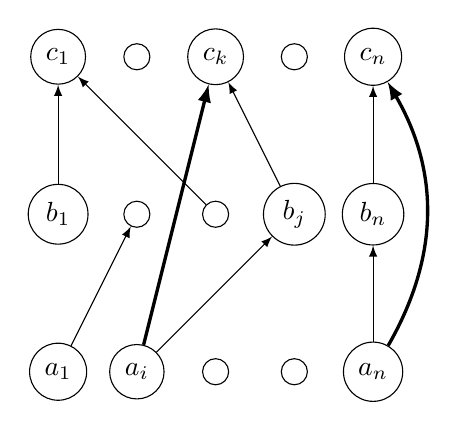
\begin{tikzpicture}
\node(A1) at (0,0) [shape=circle,draw] {$a_1$};
\node(Ai) at (1,0) [shape=circle,draw] {$a_i$};
\node at (2,0) [shape=circle,draw] {};
\node at (3,0) [shape=circle,draw] {};
\node(An) at (4,0) [shape=circle,draw] {$a_n$};
\node(B1) at (0,2) [shape=circle,draw] {$b_1$};
\node(Bw) at (2,2) [shape=circle,draw] {};
\node(Bv) at (1,2) [shape=circle,draw] {};
\node(Bj) at (3,2) [shape=circle,draw] {$b_j$};
\node(Bn) at (4,2) [shape=circle,draw] {$b_n$};
\node(C1) at (0,4) [shape=circle,draw] {$c_1$};
\node at (1,4) [shape=circle,draw] {};

\node at (3,4) [shape=circle,draw] {};
\node(Ck) at (2, 4) [shape=circle,draw] {$c_k$};
\node(Cn) at (4, 4) [shape=circle,draw] {$c_n$};


\draw[->, >=latex] (A1)--(Bv);
\draw[->, >=latex] (An)--(Bn);
\draw[->, >=latex] (Bw)--(C1);
\draw[->, >=latex] (Bn)--(Cn);
\draw[->, >=latex] (B1)--(C1);
\draw[->, >=latex] (Bj)--(Ck);
\draw[->, >=latex] (Ai)--(Bj);
%\draw[->, >=latex,plein] (A1) edge[bend left] (C1);
%\draw[->, >=latex,plein] (A1)  edge[bend right] (Cn);
\draw[->, >=latex,plein] (An) edge[bend right] (Cn);
\draw[->, >=latex,plein] (Ai)  edge[] (Ck);
%\draw[->, >=latex,plein] (An)  edge[bend right] (Cn);
\end{tikzpicture}
\caption{Structure of $X^+$, with the edges of the transitive closure in boldface}
\label{structure_closure}
\end{figure}


\begin{proof}

  We run algorithm
  \ref{transitive_closure_alg_optim},
  in time $\BigO(m^{3/2})$ by theorem
  \ref{quick_trans}, and retrieve only the edges we need, which can
  again be done in $\BigO(m)$ time (all new edges are on the beginning
  of an adjacency list, as we insert on the head of the list).
\end{proof}


\section{The transitive closure}
\paragraph{A classic algorithm}
One way to compute the transitive closure if to compute 
the APSP (all-pairs shortest 
paths) problem \todo{définir APSP, FW ?, TC <= APSP} for the graph. To do this we can use   the 
Floyd-Warshall algorithm \cite{Floyd:1962:A9S:367766.368168},
resulting in a $\BigO(n^3)$ time cost.

\paragraph{Rapid exponentiation}
If we have access to the adjacency matrix an a matric multiplication algorithm
in $\BigO(n^\alpha)$ then by using rapid exponentiation we get an algorithm
running in $\BigO(n^\alpha \log n)$, as we have that 
$X^+=\sum_{i=1}^n X^i$.

\paragraph{A more tailored approach} We can largely improve that 
result by using the following algorithm, published first in 1979
\cite{goralvcikova1979reduct}:

\begin{algorithm}
  \LinesNumbered
  \SetAlgoVlined
  \SetKwInput{Input}{Input} \SetKwInput{Output}{Output}
  \caption{computing the transitive closure of a graph}
  \label{transitive_closure_alg}
  \Input{a directed acyclic graph $G=(V,N)$, stored as a list of
    out-neighbors $N(v_i)$ for each vertex $v_i\in V$.}
  \Output{the transitive closure $G'=(V,N')$ of $G$, stored as a list
    of out-neighbors $N'(v_i)$ for each vertex $v_i \in V$.}

  Find a topological ordering $(v_1,\dots,v_n)$ of $V$\;
  \For{$i\gets n..1$}{
  $N'(v_i)\gets N(v_i)$\;
  \For{$w\in N(v_i)$}{
  $N'(v_i)\gets N'(v_i) \cup N'(w)$\;
  }}
  \textbf{return} $(V, N')$\;
\end{algorithm}
This resulted in the following
\begin{Theo}
Algorithm \ref{transitive_closure_alg} can be implemented 
in $\BigO(ns+m)$, where $s$ is the number of edges in the 
factorgraph (where all the strongly connected components
are reduced to vertices). For a DAG, this gives an algorithm
running in $\BigO(nm)$ time.
\end{Theo}

A new analysis of the algorithm has resulted in the following
improvement:

\begin{Theo}[\cite{borassi2015into}]
  It is possible to implement algorithm \ref{transitive_closure_alg} with
  time complexity $\BigO\left(n+m_{\texttt{tc}}^{3/2}\log n\right)$,
  where $m_{\texttt{tc}}$ is the number of edges in the transitive closure.
\end{Theo}

The proof uses the following lemmas:
\begin{Lemma}
\label{lemma_deg_tri}
If $n_{in}(w)$ is the in-degree of $w$ in the transitive closure
of the graph and $n_{out}(w)$ is the out-degree of $w$ in the
transitive closure, then $\sum_{w\in V}n_{in}(w)n_{out}(w)$ is
at most the number of triangles in the transitive closure, seen as
an undirected graph.
\end{Lemma}

\begin{Lemma}
\label{lemma_tri_bound}
The number of triangles in a graph with $m$ edges is at most $\BigO(m^{3/2})$.
\end{Lemma}
\begin{proof}[Proof from \cite{bound_triangles}]
Define $t(m)$ the maximum number of triangles we can form with
$m$ edges. For any complete graph, $t(m)=\BigO(m^{1.5})$ ; we have to check this holds when
${n-1 \choose 2} < m < {n\choose 2}$. Let us define $\delta$ such that
$m+\delta = {n \choose 2}$ (necessarily $\delta < m$). Then
\[ t(m) \leq t(m+\delta) = \BigO((m+\delta)^{1.5}) = \BigO((2m)^{1.5}) \]
because $t$ is non-decreasing.
\end{proof}

\begin{proof}[Proof sketch]
Line 1 is done in $\BigO(n+m)$.
Every other step apart form line 5 can be done in $\BigO(m)$ time.
The $\log n$ factor comes from line 5 where we insert new
vertices in a self-balanced binary search tree. Thus Line 5
costs $\BigO(n_{out}(w)\log n)$. Troughout a run of 
the algorithm we process a vertex $w$ in the \texttt{for} loop at
most $n_{in}(w)$ times, making the total cost of
Line 5 bounded by $\sum_{w\in V}n_{in}(w)n_{out}(w)$. Using lemmas
\ref{lemma_deg_tri} and \ref{lemma_tri_bound}, the claim follows.
\end{proof}

One can find an analysis of the algorithm on special cases in 
\cite{HABIB1993289}\todo{Utile ?}.

\subsection{Shaving off the $\log n$ factor}
We can actually do a bit better: we use tree data structures
in algorithm \ref{transitive_closure_alg} to avoid
inserting twice the same vertex in a list. We can avoid that and
use an array to keep track of what vertex has been inserted.
This only costs us a $\BigO(n)$ space
penalty, which amounts to nothing since we can assume that $n=\BigO(m)$.
This brings a positive answer to the question asked by
\cite{borassi2015into}: we can remove the $\log n$ factor. 

\begin{Theo}
%\label{quick_trans}
Algorithm \ref{transitive_closure_alg_optim} computes the transitive closure
of a graph in $\BigO(n+m^{3/2})$ time, with $m$ being the number of edges
in the transitive closure.
\end{Theo}

\begin{proof}
The loops in Line 5 and Line 12 clearly take $\BigO(m)$ time.
On Line 8, reading and setting a cell in the tab, and then inserting
a new vertex in a list are all operations done in constant time.
On Line 2, if we cannot allocate an array filled with zero in constant
time we can use a trick \cite[Exercise 2.12]{aho74} so that an unitialized cell
defaults to zero. In that case, allocate $T_1$ and $T_2$ of size $n$, 
set $p=0$ and use algorithms \ref{writing_array} and \ref{reading_array}.
\end{proof}

\begin{algorithm}
  \label{writing_array}
  \LinesNumbered
  \SetAlgoVlined
  \caption{Writing $x$ in the $i$th cell in $T$}

  $T[i] \gets x$\;
  \If{$T_2[i] > p$ or $T_1[T_2[i]] \neq i$}{
  $T_1[p] \gets i$\;
  $T_2[i] \gets p$\;
  $p \gets p +1$\;
  }
\end{algorithm}
\begin{algorithm}
  \label{reading_array}
  \LinesNumbered
  \SetAlgoVlined
  \caption{Reading the $i$th cell in $T$}
  \If{$T_2[i] > p$ or $T_1[T_2[i]] \neq i$}{
      write value 0 to $T[i]$ using algorithm \ref{writing_array}\;
  }
  return $T[i]$;
\end{algorithm}


\begin{Corol}
It is possible to check that a graph is transitive, and to check
a graph is a comparability graph, in time $\BigO(m^{3/2})$.
\end{Corol}

%\section{La fusion de liste et la réduction transitive}

\section{Transitive reduction}
\begin{Theo}[\cite{aho1972transitive}]
If there is an algorithm to compute the transitive closure of an $n$ vertex
graph in time $\BigO(n^\alpha)$, then there is an algorithm to compute 
the transitive reduction in time $\BigO(n^\alpha)$.
\end{Theo}
An important thing to note here is that the authors assume that 
one can switch from any representation to matrix form in $\BigO(n^2)$ time, 
which is a lot to ask ; the rest of the algorithm relies on 
fast multiplication algorithms. Their proof (in the case of DAGs) is as follows.
\begin{proof}[Proof sketch.]
If $A$ is the adjacency matrix of the graph, compute its transitive closure
$A^+$. Then the transitive reduction is $A-AA^+$.
\end{proof}
If we wish to adapt this algorithm to the case of sparse matrices, we can try 
to tweak our algorithm so it sees $A^+$ as a complemented representation (each
vertex has list of non-neighbors) but there does not seem to be an 
obvious way to do this (unless we use bit strings as arrays for example).
For lack of a better alternative, we have
the following bound:
\begin{Theo}
The transitive closure of a graph can be computed in
$\BigO\left(n^2 + m_{\texttt{tc}}^{3/2}\right)$ time.
\end{Theo}

This can be compared with the original algorithm of 
Goral{\v{c}}{\'{i}}kov{\'{a}} and Koubek, which runs 
in $\BigO\left(nm_{\texttt{tr}} + m_{\texttt{tc}}\right)$, where
$m_{\texttt{tr}}$ is the nujmber of edges in the transitive reduction.

\section{Existence of a triangle}
Several choices from \cite{itai1978finding} :

\paragraph{Spanning trees} 
We can use a technique based on spanning trees. 


\begin{algorithm}
  \LinesNumbered
  \SetAlgoVlined
  \SetKwInput{Input}{Input} \SetKwInput{Output}{Ouput}
  \caption{Finding whether there is a triangle}
  \label{triangle_alg}
  \Input{a directed graph $G=(V,N)$, stored as an adjacency matrix.}
  \Output{True if $G$ has a triangle, False otherwise.}

  \While{$G$ has edges}{
  Find a rooted spanning tree for each nontrivial connected components of $G$\;
  \If{Any tree edge is contained in a triangle}{
      \textbf{return} True\;
  }
  Delete the tree edges of $G$\;}
  \textbf{return} False\;
\end{algorithm}

\begin{Theo}[\cite{itai1978finding}]
This algorithm runs in $\BigO(m^{3/2})$ time.
\end{Theo}
The algorithm uses the following fact:
\begin{Lemma}{}
There exists a triangle which contains a tree edge if and only if there 
exists a nontree edge $(x,y)$ for which $(\mathrm{father}(x),y)$ is an edge.
\end{Lemma}
The proof relies on the fact we can check in constant time whether for an
nontree edge $(x,y)$, we have that $(\mathrm{father}(x),y)$ is an edge.

\paragraph{Vertex inspection}
This technique is based on the construction of the sets 
$UA(v)$: for each vertex $v$, $UA(v)$ is the list its neighbors $w$ such
that the $w > v$. This way, each edge appears only once. These lists
can be built in $O(m)$ time, and this yields a procedure
to find triangles in $\BigO(n^{5/3})$ time, and $\BigO(n^2)$ space.

\paragraph{Matrix product}
We can easily check that there is a triangle in a graph $G$ by
squaring the adjacency matrix (in which $m_{ij}=1$ if and only if
there is a path of length 2 from $i$ to $j$). Through some reduction
to directed circuits, the paper shows we can find
triangles in $\BigO(n^{\log 7})$.

\paragraph{A more recent result}
 \cite{Durand2011574} gives us the following theorem:
\begin{Theo}
Let $\beta \geq 1$ and supose that there is an algorithm that decides
whether there exists an independent size of three in a graph
in time $\BigO(m^\beta)$. Then there is an algorithm that decides whether there
exists a triangle in a graph in time $\BigO(m^{\frac{4\beta}{2\beta+1}})$.
\end{Theo}
Combining with theorem \ref{quick_indep} provides us with an algorithm that 
works in $\BigO(m^{1.19})$ time.

Using theorem \ref{fast_product} we can devise a fast combinatorial (?)
 algorithm to
check whether a graph has a triangle.
\begin{Theo}
Using our fast matrix product, we can check the existence of a triangle
in a graph $G$ given as adjacency lists in $\BigO(p^{3/2})$ where
$p$ is the number of paths of length 2 in $G$.
\end{Theo}
\begin{proof}
The matrix of $G$ being $A$, we compute $A^2$ and we check if a
vertex $v$ has a common neighbour in $A$ and $A^2$, which can be
done in a linear time in $p$.
\end{proof}
Note that by lemmas \ref{lemma_deg_tri} and \ref{lemma_tri_bound}, $p$ is
bounded by $\BigO(m_{tc}^{3/2})$ where $m_{tc}$ is
the number of edges in the transitive closure of $G$, since
the number of paths of length 2 is no greater than
$\sum_{w\in V}n_{in}(w)n_{out}(w)$.

This seems to be a more practical algorithm: although the bounds
are looser, there is no need for intricate matrix multiplication
algorithms.

\section{Existence of an independent set of size 3}
An obvious start to find an independent set would be to take the complemented
graph, and try to find a triangle in it. However as we saw, it does not seem 
easy to complement a graph given in adjacency list form.
\begin{Theo}
If there exists an algorithm that finds a triangle of size 3 running
in time $\BigO(f(n,m))$, then there is an algorithm that finds an independent
set in time $\BigO(n^2 + f(n,m))$.
\end{Theo}

%The original paper makes the assumption that we can spare a $\BigO(n^2)$ 
%time cost to switch between graph representation. As long as 
%we use a matrix representation and matrix products this is not a problem.
If we allow ourselves to use fast matrix maltiplication, we have 
\begin{Theo}[\cite{Durand2011574}]
\label{quick_indep}
There is an algorithm that either finds a 3-independent set in a graph $G$
or determines there is no such set in time $\BigO(m^{\alpha/2})$.
\end{Theo}
As a consequence there is an algorithm that finds an 3-independent set
in $\BigO(m^{1.41})$ time.



\newpage
\printbibliography
\newpage

\appendix

\section{Problem definitions}
\ProbDef{TriangleFree}{A graph $G=(V,E)$.}{\True{} if $G$ 
has no triangle, \False{} otherwise.}

\ProbDef{GraphDominatedVertex}{A graph $G=(V,E)$.}{\True{} if $G$
has a \textit{dominated vertex}, that is a vertex $v$ such that
$N(v) \subseteq N(w)$ for some $w$, \False{} otherwise.}

\ProbDef{ATFreeGraph}{A graph $G=(V,E)$.}{\True{} if $G$ does not contain
an asteroidal triple, \False{} otherwise.}

\ProbDef{GraphDominatingPair}{A graph $G=(V,E)$.}{\True{} if $G$ has a  
\textit{dominating pair}, that is a $(x,y)\in V^2$ such that for any path
$P$ from $x$ to $y$ and every vertex $z$, $z$ is adjacent to at least
one vertex of $P$, \False{} otherwise.}

\ProbDef{DominatingPair}{A graph $G=(V,E)$ and two vertices
$u$ and $v$.}{\True{} if $(u,v)$ is a dominating pair of $G$, 
\False{} otherwise.}

\ProbDef{GraphExtremities}{A graph $G=(V,E)$.}{A list of 
all the \textit{extremities} of a graph, that is all $v\in V$ such that
$G - N[v]$ is connected.\footnote{By $N[v]$ we mean the closed neighborhood
of $v$: $N[v] = \{w \in V| (v,w) \in E\}$.}}

\ProbDef{\#SimplicialVertices}{A graph $G=(V,E)$.}{The number
of \textit{simplicial vertices} of $G$, that is the number
of vertices $v$ such that $N(v)$ is a clique.}

\ProbDef{GraphTwoPair}{A graph $G=(V,E)$.}{\True{} if $G$ has
a two pair, that is a pair $(u,v)\in V^2$ such that
any chordless path between $u$ and $v$ has length two, \False{} otherwise.}

\ProbDef{GraphStarCutset}{A graph $G=(V,E)$.}{\True{} if $G$
has a \textit{star cutset}, \False{} otherwise. A star cutset
is a set $S$ of $V$ such that $G - S$ is disconnected and there is a 
$v$ in $S$ adjacent to all the other vertices in $S$.}

\ProbDef{CliqueStarCutset}{A graph $G=(V,E)$.}{\True{} if $G$
has a \textit{star cutset}, \False{} otherwise. A star cutset
is a clique $S$ of $V$ such that $G - S$ is disconnected.}

\end{document}
